
\section{Testframeworks für Ruby}
\epigraph{Ruby has laid the way in having a test-infected culture around the language}{Nathaniel Talbott (Entwickler von Test/Unit)}

Rails\index{Ruby-on-Rails} liefert standardmäßig das auf dem xUnit-Schema basierende Testframework Test/Unit\index{Test/Unit-Framwork} mit. In der Version 1.9.x bringt Ruby\index{Ruby} das Testframework Minitest in der Standardbibliothek mit, welches ebenfalls Tests nach dem xUnit-Schema unterstützt. Darüber hinaus existieren zahllose weitere Testframeworks für Ruby. Eines für den Akzeptanztest ist Cucumber, welches eine Business-readable \glossar{DSL}\footnote{Eine Domain-Spezifische-Sprache, welche durch Kunden nachvollzogen werden kann. Siehe \url{http://martinfowler.com/bliki/BusinessReadableDSL.html}} für die Definition von Spezifikationen.
\subsection{Test/Unit}
Test/Unit\index{Test/Unit-Framwork} basiert auf dem xUnit-, bzw. SUnit-Design von Kent Beck, und ist für Nutzer von z.B. JUnit oder NUnit leicht nachvollziehbar. 

Für eine zu testende Klasse wird analog eine Testklasse erstellt. Diese trägt per Definition denselben Namen wie die zu testende Klasse mit einem \texttt{Test} am Anfang. Um z.B. eine Klasse \texttt{Job} zu testen, wird eine Datei \texttt{job\_test.rb}  erstellt. Dort wiederrum wird eine Klasse mit Namen \texttt{TestJob} definiert. 


Eine solche Testklasse kann wie folgt aussehen:
\begin{ruby}[label=Testen mit Test/Unit]
\PY{n+nb}{require} \PY{l+s+s2}{"}\PY{l+s+s2}{job}\PY{l+s+s2}{"}

\PY{k}{class} \PY{n+nc}{TestJob} \PY{o}{<} \PY{n+no}{Test}\PY{o}{::}\PY{n+no}{Unit}\PY{o}{::}\PY{n+no}{TestCase}
  \PY{k}{def} \PY{n+nf}{setup}
    \PY{n+nv+vi}{@job} \PY{o}{=} \PY{n+no}{Job}\PY{o}{.}\PY{n}{create}
  \PY{k}{end}
  
  \PY{k}{def} \PY{n+nf}{teardown}
    \PY{n+no}{Job}\PY{o}{.}\PY{n}{delete\PYZus{}all}
  \PY{k}{end}
  
  \PY{k}{def} \PY{n+nf}{test\PYZus{}job\PYZus{}exists}
    \PY{n+nv+vi}{@job}\PY{o}{.}\PY{n}{title} \PY{o}{=}  \PY{l+s+s2}{"}\PY{l+s+s2}{Ruby on Rails in Entwickler}\PY{l+s+s2}{"}
    \PY{n+nv+vi}{@job}\PY{o}{.}\PY{n}{add\PYZus{}location\PYZus{}to\PYZus{}title}\PY{p}{(} \PY{l+s+s2}{"}\PY{l+s+s2}{Dresden}\PY{l+s+s2}{"}\PY{p}{)}
    
    \PY{n}{assert\PYZus{}equal}\PY{p}{(} \PY{l+s+s2}{"}\PY{l+s+s2}{Ruby on Rails Entwickler in Dresden}\PY{l+s+s2}{"}\PY{p}{,}  \PY{n+no}{Job}\PY{o}{.}\PY{n}{first}\PY{o}{.}\PY{n}{title}\PY{p}{)}
  \PY{k}{end}
\PY{k}{end}
\end{ruby}
\codecaption{Testen mit Test/Unit in Ruby}

Unsere Klasse \texttt{TestJob} erbt von der \texttt{TestUnit}-Basisklasse. Sie beinhaltet die besonderen Methoden \texttt{setup} und \texttt{teardown}, die jeweils vor, bzw. nach jedem einzelnen Testfall aufgerufen werden.
In der \texttt{setup}-Methode nehmen wir z.B. das Anlegen eines Jobs vor, in der Teardown Methode löschen wir alle Jobs in der Datenbank, um einen sauberen Test zu gewährleisten (Isolation).

Danach können nun beliebig viele Testmethoden folgen, deren Namen mit \texttt{test\_} beginnen müssen.
Jede Testmethode besteht in der Regel aus einer Initialisierung, der Ausführung einer zu testenden Aktion und dem Prüfen der danach geltenden Eigenschaften mittels Assertions. Diese Assertions, also zu Deutsch Zusicherungen, sind vom Testframework bereitgestellt Funktionen, die übergebene Parameter auf gewisse Eigenschaften testen und daraus einen Testerfolg oder Fehlschlag ableiten. Sollte eine Assertion innerhalb eines Tests fehlschlagen, so gilt der gesamte Testfall als fehlgeschlagen. \\
Einige dieser Zusicherungen sind z.B.:
\begin{description}
 \item[\texttt{assert(statement)}] Prüft, ob der angegebene Ausdruck wahr ist (In Ruby\index{Ruby} sind alle Ausdrücke, außer \texttt{false} und \texttt{nil} wahr)
 \item[\texttt{assert\_equal(expected, actually)}] prüft, ob die beiden Statements gleich sind, hinsichtlich des \texttt{==}-Operators\footnote{Viele eingebaute Klassen prüfen auf Strukturgleichheit. Eigene Objekte werden ansonsten auf Adressengleichheit getestet. Man kann allerdings eine eigene Vergleichsoperation durch die Implementation der Instanzmethode \texttt{.==()} definieren}
 
 \item[\texttt{assert\_raise(exception, \&block)}] Prüft, ob innerhalb des übergebenen Codeblocks eine Exception vom Typ exception geworfen wird
 \item[\texttt{assert\_match(regexp, string)}] Prüft, dass der Ausdruck vom Typ String dem spezifizierten regulären Ausdruck matcht
\end{description}
Natürlich lassen sich beliebige weitere Zusicherungen definieren. \glossar{rails} z.B. definiert Zusicherungen, um zu testen, ob ein Objekt eine gültige Instanz hinsichtlich der definierten Validierungen ist (Validierungen wurden bereits im Abschnitt \ref{sec:railsconcepts} erläutert).

\paragraph{Testdatengenerierung}
Nachdem Testdaten (vgl. Abschnitt \ref{sec:test}) einmal in zentraler Form definiert wurden, erledigt \glossar{rails} das Management, d.h. Laden und Löschen dieser, selbständig. Diese Art der Testdatenbereitstellung wird bei Rails \textbf{Fixtures} bezeichnet. Rails setzt selbstständig die Datenbank nach jedem einzelnen Test auf die Fixtures zurück, oder kapselt die Tests innerhalb von Transaktionen, insofern die verwendete Datenbank dies unterstützt.\\
Allerdings ist diese Form der Testdatenbereitstellung nicht unumstritten. Fixtures sind globale Daten, die in jedem Test verfügbar sind, obwohl sie nur in wenigen Testfällen benötigt werden, und machen es schwierig Grenzfälle effektiv zu definieren. Außerdem sind die Testdaten nicht in der selben Datei wie der Test zu finden, womit man Tests nur verstehen kann, wenn man die Fixtures kennt. Eine mögliche Lösung ist es, stattdessen \textbf{Factories}\footnote{http://www.dan-manges.com/blog/38} einzusetzen, die zentral Regeln definieren, wie valide Instanzen von Modellen gebaut werden. Die Tests nutzen dann die Factory um sich z.B. einen neuen Job generieren zu lassen und für den aktuellen Testfall verändern.

Zur Generierung von größeren Mengen an zufälligen Daten einer bestimmten Domän (z.B. für Stresstests) existieren ebenfalls Lösungen. Mittels der \glossarpl{gem} "`populator"' und "`faker"' lassen sich beispielsweise eine beliebige Menge an gültig-anscheinenden Personendaten (Name, Vorname, Adresse, E-Mail-Adresse, Passwort,...) oder Blind-Texten generieren\footnote{Eine sehr gute Erklärung zur Nutzung beider Gems ist im Railscast \#128 zu finden \url{http://railscasts.com/episodes/126-populating-a-database}}.


\subsection{Cucumber}
\label{sec:cucumber}
Cucumber ist ein relativ neues Framework (2008), um mittels einer domainspezifischen Sprache  (\glossar{DSL}) verständliche automatisierte Tests zu schreiben. Dabei gibt es 2 Ebenen: In der oberen werden \textit{Testschritte} in Englisch, Deutsch oder einer anderen der mehr als 30 unterstützten Sprachen spezifiziert. In der darunterliegenden werden diese Schritte in echten Testcode implementiert. \\
Im Folgenden sei ein Trivialbeispiel einer Anwendung, die Addieren implementiert, gezeigt.
\lstinputlisting[label=Cucumber: Additionsfeature in Deutsch,caption=Cucumber: Additionsfeature in Deutsch]{listings/addition.feature}
\begin{ruby}[label=addition.feature]
\PY{c}{# language: de}
\PY{n+nc}{Funktionalität}\PY{n+nc}{:}\PY{n+no}{ Addition zweier Zahlen}
\PY{n+nb}{ }\PY{n+nb}{ }\PY{n+nb}{H}\PY{n+nb}{i}\PY{n+nb}{e}\PY{n+nb}{r}\PY{n+nb}{ }\PY{n+nb}{w}\PY{n+nb}{ü}\PY{n+nb}{r}\PY{n+nb}{d}\PY{n+nb}{e}\PY{n+nb}{ }\PY{n+nb}{e}\PY{n+nb}{i}\PY{n+nb}{n}\PY{n+nb}{e}\PY{n+nb}{ }\PY{n+nb}{g}\PY{n+nb}{r}\PY{n+nb}{o}\PY{n+nb}{b}\PY{n+nb}{e}\PY{n+nb}{ }\PY{n+nb}{B}\PY{n+nb}{e}\PY{n+nb}{s}\PY{n+nb}{c}\PY{n+nb}{h}\PY{n+nb}{r}\PY{n+nb}{e}\PY{n+nb}{i}\PY{n+nb}{b}\PY{n+nb}{u}\PY{n+nb}{n}\PY{n+nb}{g}\PY{n+nb}{ }\PY{n+nb}{d}\PY{n+nb}{e}\PY{n+nb}{s}\PY{n+nb}{ }\PY{n+nb}{B}\PY{n+nb}{u}\PY{n+nb}{s}\PY{n+nb}{i}\PY{n+nb}{n}\PY{n+nb}{e}\PY{n+nb}{s}\PY{n+nb}{s}\PY{n+nb}{v}\PY{n+nb}{a}\PY{n+nb}{l}\PY{n+nb}{u}\PY{n+nb}{e}\PY{n+nb}{s}
\PY{n+nb}{ }\PY{n+nb}{ }\PY{n+nb}{u}\PY{n+nb}{n}\PY{n+nb}{d}\PY{n+nb}{ }\PY{n+nb}{d}\PY{n+nb}{e}\PY{n+nb}{r}\PY{n+nb}{ }\PY{n+nb}{R}\PY{n+nb}{a}\PY{n+nb}{h}\PY{n+nb}{m}\PY{n+nb}{e}\PY{n+nb}{n}\PY{n+nb}{b}\PY{n+nb}{e}\PY{n+nb}{d}\PY{n+nb}{i}\PY{n+nb}{n}\PY{n+nb}{g}\PY{n+nb}{u}\PY{n+nb}{n}\PY{n+nb}{g}\PY{n+nb}{e}\PY{n+nb}{n}\PY{n+nb}{ }\PY{n+nb}{s}\PY{n+nb}{t}\PY{n+nb}{e}\PY{n+nb}{h}\PY{n+nb}{e}\PY{n+nb}{n}
  \PY{n+nc}{Szenario}\PY{n+nc}{:}\PY{n+no}{ Addition von ganzen positiven Zahlen}
\PY{k}{    Wenn }ich \PY{l+s}{"}\PY{l+s}{1}\PY{l+s}{"} für a und \PY{l+s}{"}\PY{l+s}{2}\PY{l+s}{"} für b eingebe
    \PY{k}{Und }auf \PY{l+s}{"}\PY{l+s}{A}\PY{l+s}{d}\PY{l+s}{d}\PY{l+s}{i}\PY{l+s}{e}\PY{l+s}{r}\PY{l+s}{e}\PY{l+s}{n}\PY{l+s}{"} klicke
    \PY{k}{Dann }sehe ich \PY{l+s}{"}\PY{l+s}{3}\PY{l+s}{"}
\end{ruby}
\codecaption{Cucumber: Defintion eines Additionsfeature (in Deutsch)}

Wenn man nun die Datei mittels Cucumber ausführt, so wird darauf hingewiesen, dass die Testschritte noch nicht implementiert sind.

Eine Beispielimplementation (ohne Verwendung einer GUI-Anwendung) der Testschritte wäre:
\begin{ruby}[label=steps.rb]
\PY{n+no}{Wenn}\PY{l+s+sr}{ /\PYZca{}}\PY{l+s+sr}{ich "([\PYZca{}"]*)" für a und "([\PYZca{}"]*)" für b eingebe\$}\PY{l+s+sr}{/} \PY{k}{do} \PY{o}{|}\PY{n}{arg1}\PY{p}{,} \PY{n}{arg2}\PY{o}{|}
  \PY{n+nv+vi}{@addierer} \PY{o}{=} \PY{n+no}{Addierer}\PY{o}{.}\PY{n}{new}\PY{p}{(}\PY{n}{arg1}\PY{p}{,} \PY{n}{arg2}\PY{p}{)}
\PY{k}{end}

\PY{n+no}{Wenn}\PY{l+s+sr}{ /\PYZca{}}\PY{l+s+sr}{auf "([\PYZca{}"]*)" klicke\$}\PY{l+s+sr}{/} \PY{k}{do} \PY{o}{|}\PY{n}{arg1}\PY{o}{|}
  \PY{n+nv+vi}{@result} \PY{o}{=} \PY{n+nv+vi}{@addierer}\PY{o}{.}\PY{n}{add}\PY{p}{(}\PY{p}{)}
\PY{k}{end}

\PY{n+no}{Dann}\PY{l+s+sr}{ /\PYZca{}}\PY{l+s+sr}{sehe ich "([\PYZca{}"]*)"\$}\PY{l+s+sr}{/} \PY{k}{do} \PY{o}{|}\PY{n}{arg1}\PY{o}{|}
  \PY{n}{assert\PYZus{}equal}\PY{p}{(} \PY{n}{arg1}\PY{o}{.}\PY{n}{to\PYZus{}f}\PY{p}{,} \PY{n+nv+vi}{@result}\PY{p}{)}
\PY{k}{end}
 
\end{ruby}
\codecaption{Cucumber: Implementierung der Additionstestschritte in Ruby}
Die Anweisungen des Akzeptanztests werden auf die definierten Testschritte gemappt, die Cucumber dann sequentiell ausführt. 
Jeder dieser Testschritte kann nun eine beliebige Implementierung besitzen. Meist ist es entweder eine Initialisierung, eine Aktion oder eine Erwartung, ausgedrückt durch die Schlüsselwörter \texttt{Angenommen}, \texttt{Wenn} und \texttt{Dann}, bzw. \texttt{Given}, \texttt{When} und \texttt{Then} im englischen Originaldialekt. Die Einteilung in klare Testschritte fördert die Wiederverwendbarkeit der Testschritte in anderen Szenarien.

Der Vorteil von Cucumber ist nun, dass diese Feature-Datei zusammen mit dem Kunden durchgesprochen werden kann, und dass man damit an Ende eine funktionale Validierung gegenüber der Spezifikation automatisiert durchführen kann. \\ 
Cucumber ist von der Syntax so generisch, dass damit beliebige Anwendungen getestet werden, da keine Annahmen über die darunterliegende Implementierung der Testschritte gemacht wird.
Neben Ruby\index{Ruby} wird auch die Implementierung der Testschritte in Java und C\# unterstützt.

\paragraph{Testen von Webanwendungen}
Eine Einsatzmöglichkeit von Cucumber, besonders im Zusammenhang mit \glossar{rails}, ist das Testen von Webanwendungen. Dabei ist es üblich, einen Browser zu automatisieren bzw. simulieren (vgl. Abschnitt \ref{sec:acceptance}), um den Test so authentisch am echten Nutzungsprozess wie möglich zu orientieren. 

Um unsere Tests von der Steuerung eines konkreten Browsers unabhängig zu machen, verwenden wir verschiedene Middlewars. Wir haben uns für Capybara entschieden, welches sehr flexibel bei der Wahl der Browser-Engine ist. Den eigentlichen Test, d.h. die Auswertung der Zusicherung kann durch ein beliebiges Testframework durchgeführt werden, in unserem Falle wieder mit Test/Unit\index{Test/Unit-Framwork}. Durch Capybara haben wir nun die Möglichkeit, zwischen einem simulierten Browser (z.B. RackTest) und automatisierten Browser (Firefox, Chrome, etc. durch eine weitere Middleware: Selenium\index{Selenium}) je nach Bedarf zu wechseln, ohne viele am Testcode zu ändern.
\begin{figure}[htbp]
 \centering
 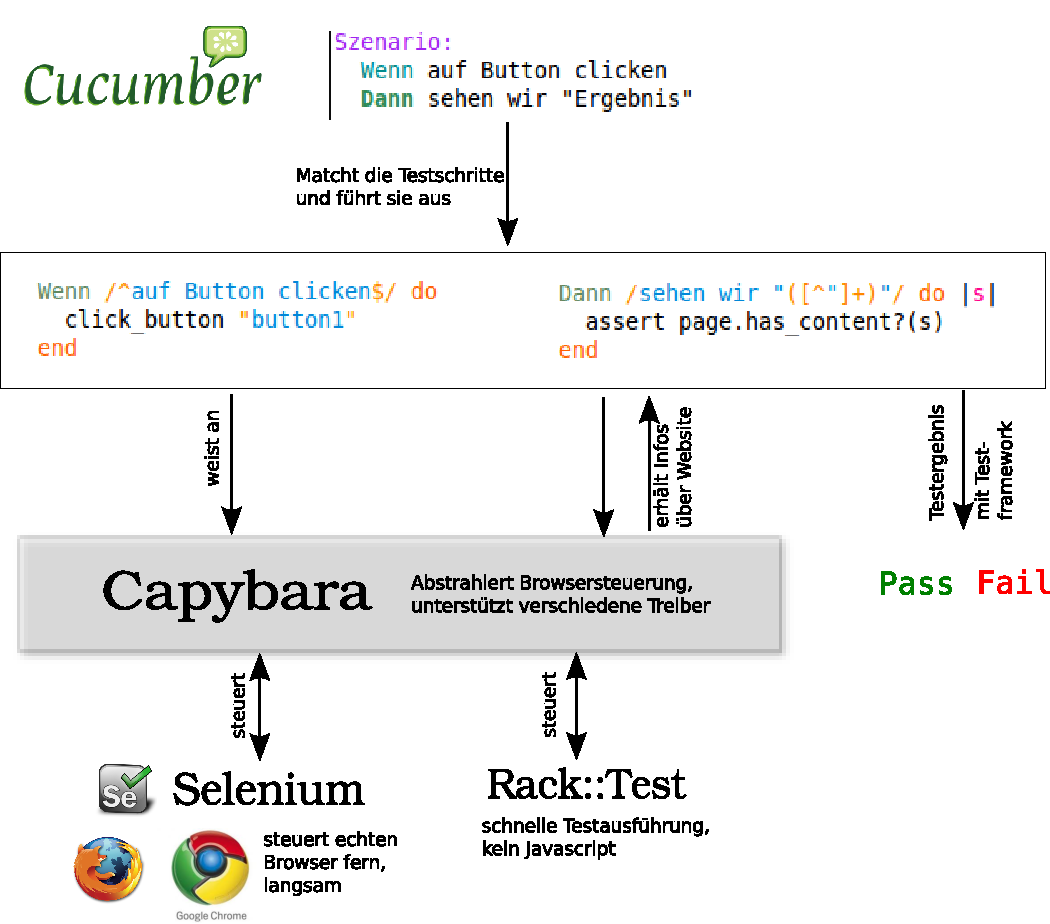
\includegraphics[width=\linewidth]{./diagrams/cucumber.pdf}
 % cucumber.pdf: 595x842 pixel, 72dpi, 20.99x29.70 cm, bb=
 \caption{Ablauf beim Akzeptanztest mit Cucumber und Capybara}
 \label{fig:cucumber}
\end{figure}

Der gesamte Ablauf eines CucumberAkzeptanztest in Verbindung mit Capybara ist in Abbildung \ref{fig:cucumber} abgebildet. Cucumber matcht die definierten Testanweisungen auf die Testschritte, und führt den darin enthalten Code aus. Dies kann zum einen die Steuerung eines Webbrowsers durch Capybara sein, oder zum anderen eine Zusicherung.
